%\documentclass[12pt,a4paper,oneside,openany]{memoir} 
% Skabelon af DTU's LaTeX support gruppe, v20090423

\usepackage[utf8]{inputenc} 
%\usepackage[danish]{babel} % danske overskrifter
\usepackage[T1]{fontenc}   % fonte (output)
\usepackage{lmodern}       % vektor fonte
\usepackage{fancybox, graphicx}      % indsættelse af billeder
\usepackage{palatino}      % lækker font
\usepackage{pdfpages}      % pdf som forside evt
\usepackage{todonotes}
\usepackage{microtype}
% \linespread{1.3}           % kræver lidt mere line spacing

\newcommand{\code}[1]{\texttt{#1}}
\newcommand{\HRule}{\rule{\linewidth}{0.5mm}}

%\addto\captionsdanish{
%  \renewcommand{\contentsname}%
%    {Indholdsfortegnelse}     %
%} % Så bruger vi bare 'Indholdsfortegnelse' i stedet for 'Indhold'


\usepackage{underscore}
\usepackage{pdflscape}
\usepackage{todonotes}

\usepackage[plainpages=false,pdfpagelabels,pageanchor=false]{hyperref} % aktive links
\def\sectionautorefname{afsnit}

\usepackage{memhfixc}  % rettelser til hyperref

\usepackage{tipa}
\pretolerance=2500     % højt tal, mindre orddeling og mere space mellem ord.
% 3000 er okey, 1000 er for lidt, 5000 i overkanten, 8000 er for meget..

\usepackage[font=small,labelfont=bf,labelsep=endash]{caption}
 
\pagestyle{headings}


\makechapterstyle{mortenovi}{%
\setlength{\beforechapskip}{0cm}%længde fra top af side til kapitel-overskrifter
\setlength{\afterchapskip}{1cm}%længde fra kapiteltekst til body-tekst
\setlength{\midchapskip}{2cm}%længe mellem kapitelnummer og kapiteltekst
\renewcommand\chapnamefont{\normalfont\Large\scshape\raggedleft}
\renewcommand\chaptitlefont{\normalfont\Huge\bfseries\sffamily}
\renewcommand\chapternamenum{}%default "kapitel"
\renewcommand\printchapternum{%
    \makebox[0pt][l]{%
    \hspace{0.4em}
    \resizebox{!}{4ex}{\chapnamefont\bfseries\sffamily\thechapter}}
    }%"kapitel. x"-linjen og dens boxe og bredder - prøv at sætte xyz ind først på de tre linjer respektivt.
\renewcommand\afterchapternum{\par\hspace{1.5cm}\hrule\vspace{0.5cm}}
\renewcommand\afterchaptertitle{\vskip\onelineskip \hrule\vskip\afterchapskip
}}
\chapterstyle{mortenovi}

\maxtocdepth{subsection} %Only parts, chapters and sections in the table of contents
\settocdepth{subsection}

% \includeonly{forord,testing} % Kompiler kun de kapitler du arbejder med.

\usepackage{listings}
\usepackage{color}

\renewcommand*\lstlistingname{Kode}

\definecolor{dkgreen}{rgb}{0,0.6,0}
\definecolor{gray}{rgb}{0.5,0.5,0.5}
\definecolor{mauve}{rgb}{0.58,0,0.82}

\lstset{frame=tb, %lr
  language=Java,
  aboveskip=3mm,
  belowskip=3mm,
  showstringspaces=false,
  columns=flexible,
  basicstyle={\small\ttfamily},
  numbers=none,
  numberstyle=\tiny\color{gray},
  keywordstyle=\color{blue},
  commentstyle=\color{dkgreen},
  stringstyle=\color{mauve},
  breaklines=true,
  breakatwhitespace=true,
  basicstyle=\tiny\ttfamily
}

\usepackage{cleveref}


\begin{document}
%\includepdf[fitpaper]{billeder/forside}


\begin{center}
\thispagestyle{empty}

% Upper part of the page. The '~' is needed because \\
% only works if a paragraph has started.

\textsc{\LARGE IT University of Copenhagen}\\[1.5cm]

\textsc{\Large BDSA 2014 }\\[0.5cm]

% Title
\HRule \\[0.4cm]
{ \huge \bfseries Calendar System \\ System Design Document\\ [0.4cm]
    %\large \\ [0.4cm] 
    }

\HRule \\[1cm]

\textsc{\Large Assignment 40 }\\[1.5cm]

% Author and supervisor
\begin{minipage}{1\textwidth}
\begin{center} \large
Anders Wind Steffensen - awis@itu.dk\\
Christopher Blundell - ppma@itu.dk\\
Pierre Mandas - cnbl@itu.dk\\
\end{center}
\end{minipage}


\vfill

% Bottom of the page
{\large \today}

\end{center}

\frontmatter%

%\include{abastract}
%\include{preface}

%\tableofcontents* % stjernen betyder vi ikke har den med i vores indholdsfortegnelse

\tableofcontents
\newpage

\mainmatter%

%input chapters here

\chapter{Introduction}

\section{Purpose of the system}
\section{Scope of the system}
The system will be created over a short amount of time and therefore will have some limitations.\\
Features
\begin{itemize}
\item Create event
\item Edit event
\item Two kinds of overview of events: Monthly and Weekly
\item Notifications
\item Get local time from global time.
\item Filter events by tags.
\item Get access to events from any Windows 7 or 8 pc
\end{itemize}
\section{Objectives and succes criteria of the project}
\section{Definitions, acronyms and abbrevations}
\section{References}
\emph{None at the time.}
\section{Overview}
The architecture of the Calendar system will be centered around a model view controller pattern, and since data persistance is neccecary four ideal subsystems come inot mind.\\
Controller, View, Model and datastorage subsystems. Each of these systems have a specific role and by using these subsystems we loosen the coupling and increase the coherence.
\chapter{Current Software Architecture}
\chapter{Proposed Software Architecture}

\section{Overview}
\textbf{View subsystem:}
This subsystem contains the different types of views that will show, depending on how the user is 
using the system. Therefore, its assignment of functionality will be that this subsystem 
has to keep track of the different views.\\
\textbf{Model subsystem:}
This subsystem contains the data that the system will be using. When the model changes state, 
it will notify the controllers, and the controllers will then change the view. Therefore, 
this subsystems assignment of functionality will be notifying the controllers, 
when its state is being changed.\\
\textbf{Controller subsystem:}
This subsystem is being used to update the views, by receiving the models state. 
Its assignment of functionality will be that this subsystem will have to update the views 
with the received models state.\\
\textbf{DataStorage subsystem:}
The DataStorage subsystem creates persistance of data either through a Database connection or locally in a file storage. The Client can gain access to the storage through a storage client which controls which kind of storage must be used at a given time and also controls the logic for the model to storage convertion. 

\subsection{Overview of the program}
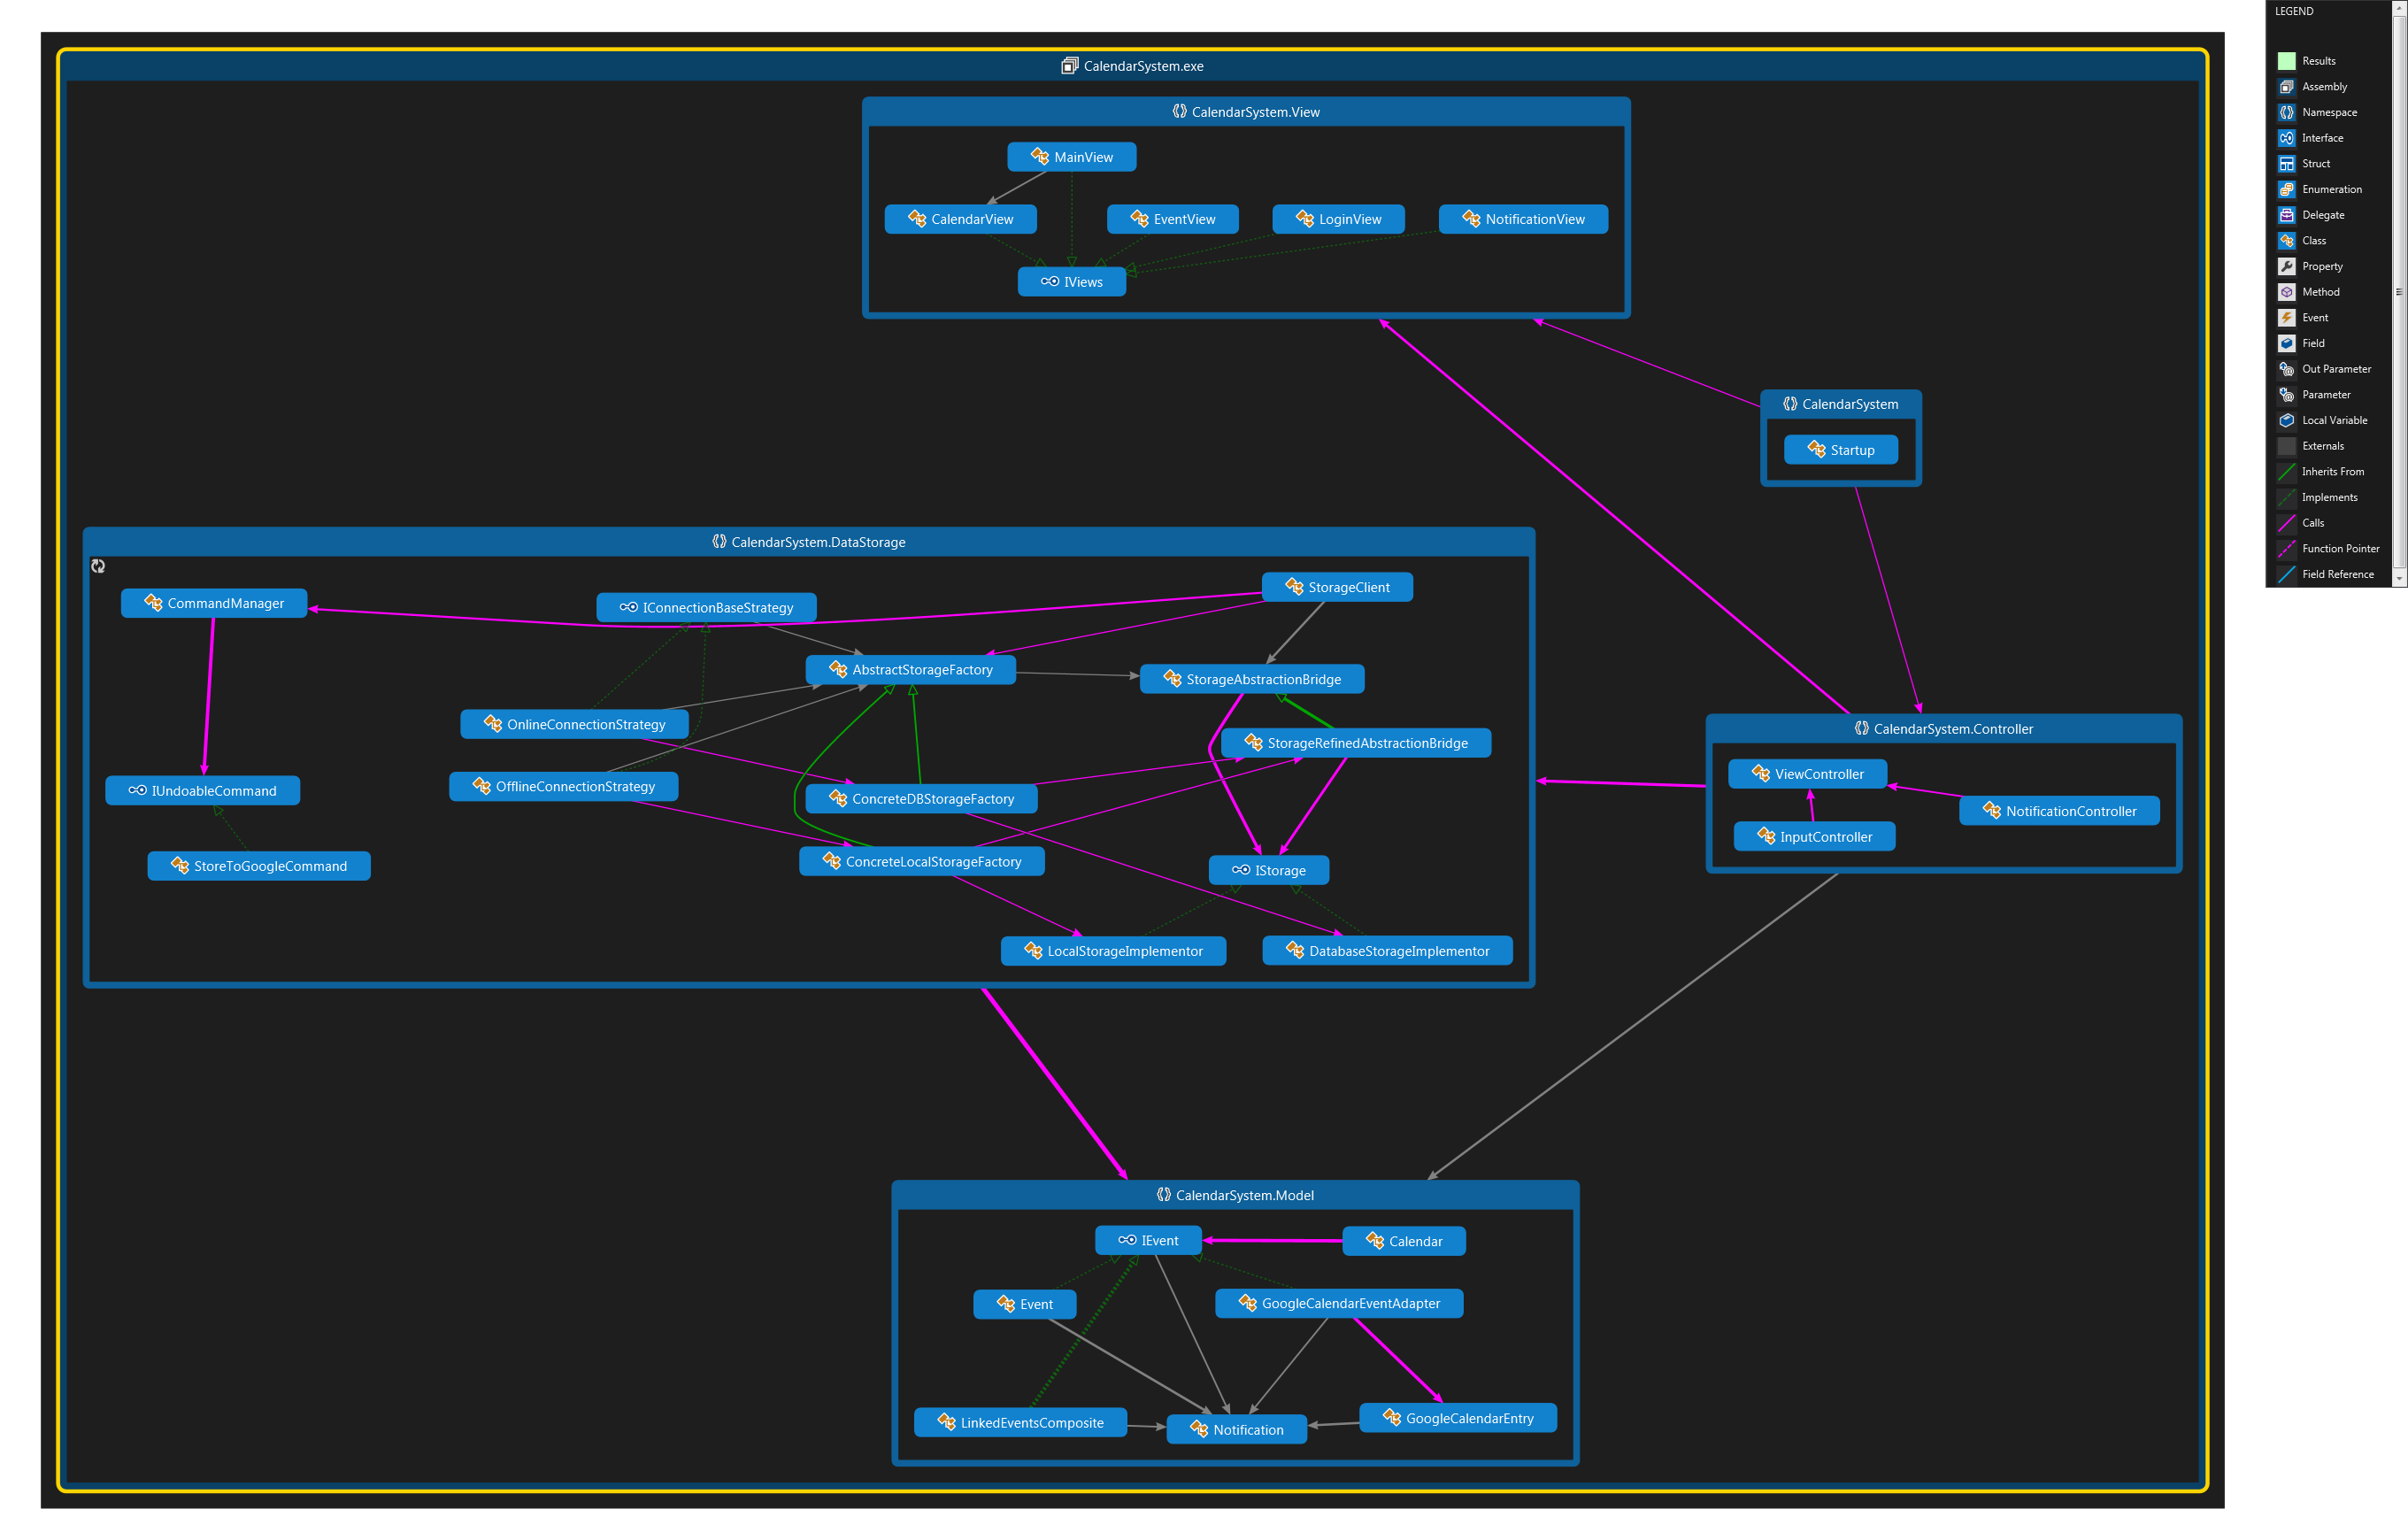
\includegraphics[scale=0.13]{OverallClassDependencies}\\

The figure shows the overall dependencies of the system, which object refers to which. References between objects in the subsystems are not included. In the Model Subsystem the objects form the data we want represented. Events, notifications, and so on. \\There are also a few extra classes the LinkedEventsComposite which is part of a Composite pattern used for linking together events, and the GoogleCalendarEventAdapter which is part of an Adapter pattern to make GoogleCalendarEvents able to be used along side our systems events.

The other interesting subsystem is the DataStorage. The classes of the subsystem form a number of objects which are used to store data. The objects form a number of design patterns together: The classes which is suffixed with Strategy forms a strategy pattern used to choose which factory to use. \\The classes suffixed with Factory is part of the Abstract factory pattern. These factories creates the products LocalStorageImplementor and DatabaseStorageImplementor in a bridge pattern class (suffixed with Bridge). \\The classes containing Command in their name are part of a command pattern, here the CommandManager can hold a number of commands, execute them and in case of a failure, call the commands undo method.\\

The classes in the subsystems Controller and View do not contain any design patterns.
\section{Subsystem decomposition}

We have chosen to use the MVC design pattern, to make a clear distinction of what functionality 
should be assigned to which part of our system. The MVC pattern stands for Model-View-Control, 
and it’s commonly used for implementing user interfaces.
\\\\
We have also chosen to create a database, whereas this database will be used to store persistent data, to when the user will logout or close the program. This will make it possible to receive earlier used data.

As we have chosen to use the MVC pattern, we will have 3 different subsystems, plus the subsystem of our database storage:

\begin{itemize}
	\item Model
	\item View
	\item Control
	\item DataStorage
\end{itemize}

The overall relations between the subsystems can be seen here. The controller controls the flow of the software and takes requests and sends data on from the storage. Objects from the Model will be send to the controller and in some cases the view, from the storage.\newpage
\textbf{Overall Subsystem Decomposition}\\
\begin{figure}[h!]
	\centering
		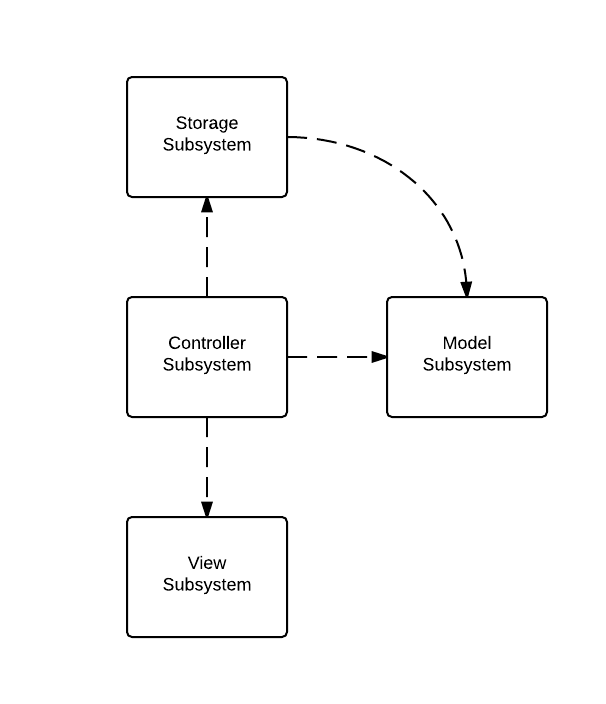
\includegraphics[scale=0.8]{OverallSubsystemDecomposition}
	\caption{The overall subsystem decomposition - not up-to-date}
  \label{fig:OverallSubsystemDecomposition}
\end{figure}

Our \textbf{Model subsystem} has the responsibility to keep notifying the controllers to update the views, which the user is using. Here is a picture of our subsystem:\\
\begin{figure}[h!]
	\centering
		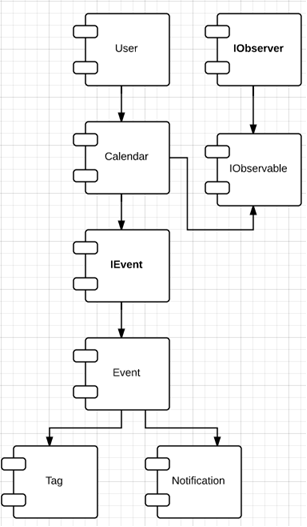
\includegraphics[scale=0.8]{modelSubsystem}
		\caption{The model subsystem decomposition - not up-to-date}
  \label{fig:ModelSubsystemDecomposition}
\end{figure}
\pagebreak

Our \textbf{View subsystem} has the responsibility to represent the model’s state. Whenever the state of the model is changed, the view will also be changed to represent the new state of the model. Here is a picture of our subsystem:\\
\begin{figure}[h!]
	\centering
		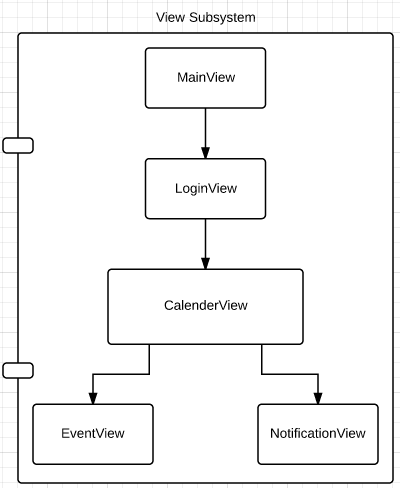
\includegraphics[scale=0.8]{viewSubsystem}
	\caption{The view subsystem decomposition}
  \label{fig:ViewSubsystemDecomposition}
\end{figure}
\\

Our \textbf{Control subsystem} has the responsibility to update the view, whenever the model has changed. The controllers will be used to update the views, by being notified by the model about its state. Here is a picture of subsystem:\\
\begin{figure}[h!]
	\centering
		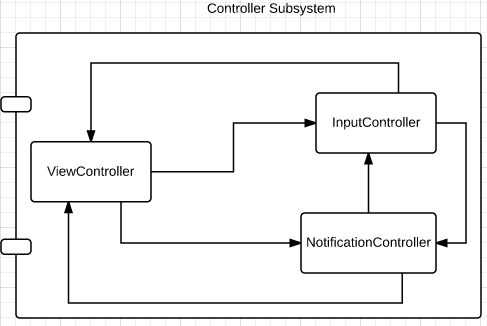
\includegraphics[scale=0.8]{controlSubsystem}
	\caption{The control subsystem decomposition}
  \label{fig:ControlSubsystemDecomposition}
\end{figure}

\pagebreak

Our \textbf{DataStorage subsystem} has the responsibility to save persistent data, which the system will be using at another time. Persistent data could be a calendar for a specific user. When the user will be login into the system, the controllers will be using the DataStorage subsystem to receive the calendar. Here is a picture of our subsystem:\\
\begin{figure}[h!]
	\centering
		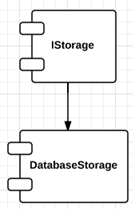
\includegraphics[scale=0.8]{datastorageSubsystem}
	\caption{The data control subsystem decomposition - not up to date}
  \label{fig:DataStorageSubsystemDecomposition}
\end{figure}
\newpage
\section{Hardware/software mapping}
\textbf{Hardware/Software Mapping}\\
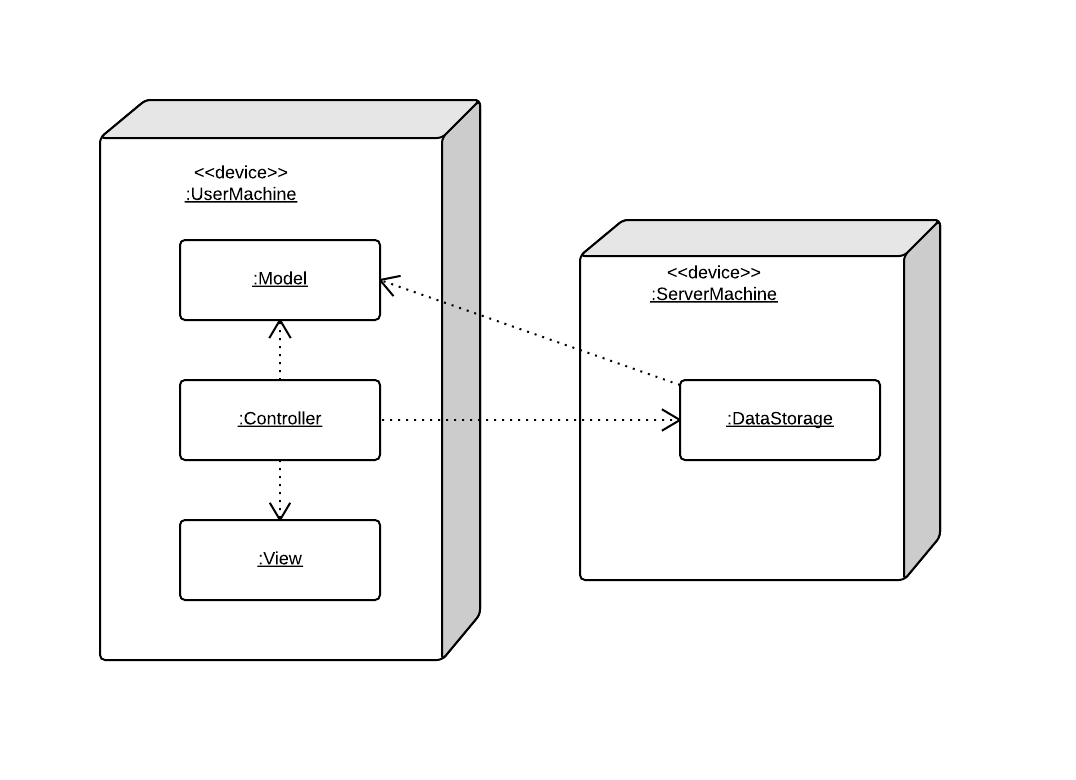
\includegraphics[scale=0.4]{HardwareSoftwareMapping}\\\\
The three subsystems running on the UserMachine are Model, Controller and View. The Controller interacts both with the Model and the View, for logic and presentation. Upon saving an event in the CalendarSystem, the Controller will then communicate with the second device, the ServerMachine, and send/request data. Following this, the DataStorage returns the data to the Model and can be done with as pleased.
\section{Persistent data management}
To save the data in form of events, tags and so on, an online database connection will be used. The database gives access to data quickly and from multiple locations. The problem with this solution is that it requires an internet connection. To work around this a strategy design pattern can be implemented to provide the application the possibility to store data locally if no connection is available and vice. versa. \\
To peek, post, update, delete LINQ can be used since it supports these features in a strong cross storage-platform language.
\section{Access control and security}

\textbf{Access Matrix for CalendarSystem}\\\\
\linethickness{1pt}
\setlength{\arrayrulewidth}{1pt}
\begin{tabular}{|c|c|c|c|}
    \hline
    \backslashbox{Actors}{Objects} & Calendar  & Notification & Event \\ \hline
               User & createCalendar & setNotification & createEvent\\
            & updateCalendar &  & updateEvent\\
            & deleteCalendar &  & deleteEvent \\
            & userLogin & & \\ \hline
                 System & createCalendarView & createNotifier &createEventView  \\ \hline
\end{tabular}\\\\

Due to the fact that our Calendarsystem is available for many users, possibly with sensitive information, it is important to keep the individuals data private as seen necessary. This is done by providing each user with a password. When the user wishes to access his or her data, the password will be prompted, and after authentication through encryption, the respective data will be accessable to the user. This limits the users access to other users personal information.\\
Furthermore it can bee seen from the matrix that the user only has access to certain data through certain objects. This is done to provide ease of use to the user. While the user can create, delete and update entries and modify their associations, the system handles the automated `reminders'.

%\end{document}

\section{Global software control}
%To ensure safe threading, concurrent data access some design choices have to be made therefore:
%\begin{itemize}
%\item The boundary objects in the view subsystem should not define any fields or change any data only show it. Therefore the view should only handle temporary objects or simple data types from the objects.
%\item Classes should provide getters and setters for their objects, but never allow for direct access to the field.
%\end{itemize}

\section{Boundary conditions}
When looking at the data storage a boundary use case stands clear. If the storage must be able to save data locally and in the cloud(online database), the storage must have a method which can check for data integrity between the two, such that the online database at all possible time has the newest data.\\

When looking at the start and shutdown of the system, making sure that data is saved and retrieved to/from the available storage(optimally the online database).
\section{Interfaces}

\textbf{IViews\\}
An interface containing three central methods, common for all our views that implement this interface:
Show();
Hide();
Clear();\\\\
\textbf{IEvent\\}
An interface made for the event class. This interface contains methods which hold the bare minimum that an Event should be able to do.\\\\
\textbf{INotification\\}
An inferface made for the notification class. This interface contains a method for setting the description of a notification, and a method for determining whether or not the notification is in an alarm state.\\\\
\textbf{IStorage\\}
An interface for the storage class. The interface has methods which makes it possible to retrieve and save events into the calendar, without knowing the actual implementation.
\chapter{Subsystem Services}
\textbf{Subsystem Services}\\\\
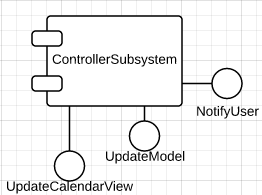
\includegraphics[scale=0.8]{ControllerServices}\\\\
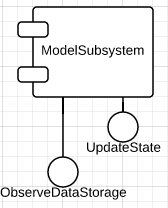
\includegraphics[scale=0.8]{ModelServices}\\\\
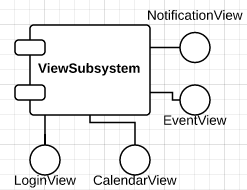
\includegraphics[scale=0.8]{ViewServices}\\\\
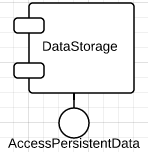
\includegraphics[scale=0.8]{DatastorageServices}\\\\
\chapter{Glossary}


\end{document}